%%
% Copyright (c) 2017 - 2021, Pascal Wagler;
% Copyright (c) 2014 - 2021, John MacFarlane
%
% All rights reserved.
%
% Redistribution and use in source and binary forms, with or without
% modification, are permitted provided that the following conditions
% are met:
%
% - Redistributions of source code must retain the above copyright
% notice, this list of conditions and the following disclaimer.
%
% - Redistributions in binary form must reproduce the above copyright
% notice, this list of conditions and the following disclaimer in the
% documentation and/or other materials provided with the distribution.
%
% - Neither the name of John MacFarlane nor the names of other
% contributors may be used to endorse or promote products derived
% from this software without specific prior written permission.
%
% THIS SOFTWARE IS PROVIDED BY THE COPYRIGHT HOLDERS AND CONTRIBUTORS
% "AS IS" AND ANY EXPRESS OR IMPLIED WARRANTIES, INCLUDING, BUT NOT
% LIMITED TO, THE IMPLIED WARRANTIES OF MERCHANTABILITY AND FITNESS
% FOR A PARTICULAR PURPOSE ARE DISCLAIMED. IN NO EVENT SHALL THE
% COPYRIGHT OWNER OR CONTRIBUTORS BE LIABLE FOR ANY DIRECT, INDIRECT,
% INCIDENTAL, SPECIAL, EXEMPLARY, OR CONSEQUENTIAL DAMAGES (INCLUDING,
% BUT NOT LIMITED TO, PROCUREMENT OF SUBSTITUTE GOODS OR SERVICES;
% LOSS OF USE, DATA, OR PROFITS; OR BUSINESS INTERRUPTION) HOWEVER
% CAUSED AND ON ANY THEORY OF LIABILITY, WHETHER IN CONTRACT, STRICT
% LIABILITY, OR TORT (INCLUDING NEGLIGENCE OR OTHERWISE) ARISING IN
% ANY WAY OUT OF THE USE OF THIS SOFTWARE, EVEN IF ADVISED OF THE
% POSSIBILITY OF SUCH DAMAGE.
%%

%%
% This is the Eisvogel pandoc LaTeX template.
%
% For usage information and examples visit the official GitHub page:
% https://github.com/Wandmalfarbe/pandoc-latex-template
%%

% Options for packages loaded elsewhere
\PassOptionsToPackage{unicode}{hyperref}
\PassOptionsToPackage{hyphens}{url}
\PassOptionsToPackage{dvipsnames,svgnames*,x11names*,table}{xcolor}
%
\documentclass[
  paper=a4,
  ,captions=tableheading
]{scrartcl}
\usepackage{amsmath,amssymb}
\usepackage{lmodern}
\usepackage{setspace}
\setstretch{1.2}
\usepackage{ifxetex,ifluatex}
\ifnum 0\ifxetex 1\fi\ifluatex 1\fi=0 % if pdftex
  \usepackage[T1]{fontenc}
  \usepackage[utf8]{inputenc}
  \usepackage{textcomp} % provide euro and other symbols
\else % if luatex or xetex
  \usepackage{unicode-math}
  \defaultfontfeatures{Scale=MatchLowercase}
  \defaultfontfeatures[\rmfamily]{Ligatures=TeX,Scale=1}
  \setmainfont[]{SF Pro Display}
  \setsansfont[]{SF Pro Display Bold}
  \setmonofont[]{Fira Code Retina}
\fi
% Use upquote if available, for straight quotes in verbatim environments
\IfFileExists{upquote.sty}{\usepackage{upquote}}{}
\IfFileExists{microtype.sty}{% use microtype if available
  \usepackage[]{microtype}
  \UseMicrotypeSet[protrusion]{basicmath} % disable protrusion for tt fonts
}{}
\makeatletter
\@ifundefined{KOMAClassName}{% if non-KOMA class
  \IfFileExists{parskip.sty}{%
    \usepackage{parskip}
  }{% else
    \setlength{\parindent}{0pt}
    \setlength{\parskip}{6pt plus 2pt minus 1pt}}
}{% if KOMA class
  \KOMAoptions{parskip=half}}
\makeatother
\usepackage{xcolor}
\definecolor{default-linkcolor}{HTML}{A50000}
\definecolor{default-filecolor}{HTML}{A50000}
\definecolor{default-citecolor}{HTML}{4077C0}
\definecolor{default-urlcolor}{HTML}{4077C0}
\IfFileExists{xurl.sty}{\usepackage{xurl}}{} % add URL line breaks if available
\IfFileExists{bookmark.sty}{\usepackage{bookmark}}{\usepackage{hyperref}}
\hypersetup{
  pdftitle={Reproducible Research: Peer Assessment 1},
  hidelinks,
  breaklinks=true,
  pdfcreator={LaTeX via pandoc with the Eisvogel template}}
\urlstyle{same} % disable monospaced font for URLs
\usepackage[margin=2.5cm,includehead=true,includefoot=true,centering,]{geometry}
\usepackage{color}
\usepackage{fancyvrb}
\newcommand{\VerbBar}{|}
\newcommand{\VERB}{\Verb[commandchars=\\\{\}]}
\DefineVerbatimEnvironment{Highlighting}{Verbatim}{commandchars=\\\{\}}
% Add ',fontsize=\small' for more characters per line
\usepackage{framed}
\definecolor{shadecolor}{RGB}{248,248,248}
\newenvironment{Shaded}{\begin{snugshade}}{\end{snugshade}}
\newcommand{\AlertTok}[1]{\textcolor[rgb]{0.94,0.16,0.16}{#1}}
\newcommand{\AnnotationTok}[1]{\textcolor[rgb]{0.56,0.35,0.01}{\textbf{\textit{#1}}}}
\newcommand{\AttributeTok}[1]{\textcolor[rgb]{0.77,0.63,0.00}{#1}}
\newcommand{\BaseNTok}[1]{\textcolor[rgb]{0.00,0.00,0.81}{#1}}
\newcommand{\BuiltInTok}[1]{#1}
\newcommand{\CharTok}[1]{\textcolor[rgb]{0.31,0.60,0.02}{#1}}
\newcommand{\CommentTok}[1]{\textcolor[rgb]{0.56,0.35,0.01}{\textit{#1}}}
\newcommand{\CommentVarTok}[1]{\textcolor[rgb]{0.56,0.35,0.01}{\textbf{\textit{#1}}}}
\newcommand{\ConstantTok}[1]{\textcolor[rgb]{0.00,0.00,0.00}{#1}}
\newcommand{\ControlFlowTok}[1]{\textcolor[rgb]{0.13,0.29,0.53}{\textbf{#1}}}
\newcommand{\DataTypeTok}[1]{\textcolor[rgb]{0.13,0.29,0.53}{#1}}
\newcommand{\DecValTok}[1]{\textcolor[rgb]{0.00,0.00,0.81}{#1}}
\newcommand{\DocumentationTok}[1]{\textcolor[rgb]{0.56,0.35,0.01}{\textbf{\textit{#1}}}}
\newcommand{\ErrorTok}[1]{\textcolor[rgb]{0.64,0.00,0.00}{\textbf{#1}}}
\newcommand{\ExtensionTok}[1]{#1}
\newcommand{\FloatTok}[1]{\textcolor[rgb]{0.00,0.00,0.81}{#1}}
\newcommand{\FunctionTok}[1]{\textcolor[rgb]{0.00,0.00,0.00}{#1}}
\newcommand{\ImportTok}[1]{#1}
\newcommand{\InformationTok}[1]{\textcolor[rgb]{0.56,0.35,0.01}{\textbf{\textit{#1}}}}
\newcommand{\KeywordTok}[1]{\textcolor[rgb]{0.13,0.29,0.53}{\textbf{#1}}}
\newcommand{\NormalTok}[1]{#1}
\newcommand{\OperatorTok}[1]{\textcolor[rgb]{0.81,0.36,0.00}{\textbf{#1}}}
\newcommand{\OtherTok}[1]{\textcolor[rgb]{0.56,0.35,0.01}{#1}}
\newcommand{\PreprocessorTok}[1]{\textcolor[rgb]{0.56,0.35,0.01}{\textit{#1}}}
\newcommand{\RegionMarkerTok}[1]{#1}
\newcommand{\SpecialCharTok}[1]{\textcolor[rgb]{0.00,0.00,0.00}{#1}}
\newcommand{\SpecialStringTok}[1]{\textcolor[rgb]{0.31,0.60,0.02}{#1}}
\newcommand{\StringTok}[1]{\textcolor[rgb]{0.31,0.60,0.02}{#1}}
\newcommand{\VariableTok}[1]{\textcolor[rgb]{0.00,0.00,0.00}{#1}}
\newcommand{\VerbatimStringTok}[1]{\textcolor[rgb]{0.31,0.60,0.02}{#1}}
\newcommand{\WarningTok}[1]{\textcolor[rgb]{0.56,0.35,0.01}{\textbf{\textit{#1}}}}

% Workaround/bugfix from jannick0.
% See https://github.com/jgm/pandoc/issues/4302#issuecomment-360669013)
% or https://github.com/Wandmalfarbe/pandoc-latex-template/issues/2
%
% Redefine the verbatim environment 'Highlighting' to break long lines (with
% the help of fvextra). Redefinition is necessary because it is unlikely that
% pandoc includes fvextra in the default template.
\usepackage{fvextra}
\DefineVerbatimEnvironment{Highlighting}{Verbatim}{breaklines,fontsize=\small,commandchars=\\\{\}}

% add backlinks to footnote references, cf. https://tex.stackexchange.com/questions/302266/make-footnote-clickable-both-ways
\usepackage{footnotebackref}
\usepackage{graphicx}
\makeatletter
\def\maxwidth{\ifdim\Gin@nat@width>\linewidth\linewidth\else\Gin@nat@width\fi}
\def\maxheight{\ifdim\Gin@nat@height>\textheight\textheight\else\Gin@nat@height\fi}
\makeatother
% Scale images if necessary, so that they will not overflow the page
% margins by default, and it is still possible to overwrite the defaults
% using explicit options in \includegraphics[width, height, ...]{}
\setkeys{Gin}{width=\maxwidth,height=\maxheight,keepaspectratio}
% Set default figure placement to htbp
\makeatletter
\def\fps@figure{htbp}
\makeatother
\setlength{\emergencystretch}{3em} % prevent overfull lines
\providecommand{\tightlist}{%
  \setlength{\itemsep}{0pt}\setlength{\parskip}{0pt}}
\setcounter{secnumdepth}{-\maxdimen} % remove section numbering

% Make use of float-package and set default placement for figures to H.
% The option H means 'PUT IT HERE' (as  opposed to the standard h option which means 'You may put it here if you like').
\usepackage{float}
\floatplacement{figure}{H}

\ifluatex
  \usepackage{selnolig}  % disable illegal ligatures
\fi

\title{Reproducible Research: Peer Assessment 1}
\author{}
\date{}



%%
%% added
%%

%
% language specification
%
% If no language is specified, use English as the default main document language.
%

\ifnum 0\ifxetex 1\fi\ifluatex 1\fi=0 % if pdftex
  \usepackage[shorthands=off,main=english]{babel}
\else
      % load polyglossia as late as possible as it *could* call bidi if RTL lang (e.g. Hebrew or Arabic)
  \usepackage{polyglossia}
  \setmainlanguage[]{english}
\fi



%
% for the background color of the title page
%

%
% break urls
%
\PassOptionsToPackage{hyphens}{url}

%
% When using babel or polyglossia with biblatex, loading csquotes is recommended
% to ensure that quoted texts are typeset according to the rules of your main language.
%
\usepackage{csquotes}

%
% captions
%
\definecolor{caption-color}{HTML}{777777}
\usepackage[font={stretch=1.2}, textfont={color=caption-color}, position=top, skip=4mm, labelfont=bf, singlelinecheck=false, justification=raggedright]{caption}
\setcapindent{0em}

%
% blockquote
%
\definecolor{blockquote-border}{RGB}{221,221,221}
\definecolor{blockquote-text}{RGB}{119,119,119}
\usepackage{mdframed}
\newmdenv[rightline=false,bottomline=false,topline=false,linewidth=3pt,linecolor=blockquote-border,skipabove=\parskip]{customblockquote}
\renewenvironment{quote}{\begin{customblockquote}\list{}{\rightmargin=0em\leftmargin=0em}%
\item\relax\color{blockquote-text}\ignorespaces}{\unskip\unskip\endlist\end{customblockquote}}

%
% Source Sans Pro as the de­fault font fam­ily
% Source Code Pro for monospace text
%
% 'default' option sets the default
% font family to Source Sans Pro, not \sfdefault.
%
\ifnum 0\ifxetex 1\fi\ifluatex 1\fi=0 % if pdftex
    \usepackage[default]{sourcesanspro}
  \usepackage{sourcecodepro}
  \else % if not pdftex
    \fi

%
% heading color
%
\definecolor{heading-color}{RGB}{40,40,40}
\addtokomafont{section}{\color{heading-color}}
% When using the classes report, scrreprt, book,
% scrbook or memoir, uncomment the following line.
%\addtokomafont{chapter}{\color{heading-color}}

%
% variables for title, author and date
%
\usepackage{titling}
\title{Reproducible Research: Peer Assessment 1}
\author{}
\date{}

%
% tables
%

%
% remove paragraph indention
%
\setlength{\parindent}{0pt}
\setlength{\parskip}{6pt plus 2pt minus 1pt}
\setlength{\emergencystretch}{3em}  % prevent overfull lines

%
%
% Listings
%
%


%
% header and footer
%
\usepackage{fancyhdr}

\fancypagestyle{eisvogel-header-footer}{
  \fancyhead{}
  \fancyfoot{}
  \lhead[]{Reproducible Research: Peer Assessment 1}
  \chead[]{}
  \rhead[Reproducible Research: Peer Assessment 1]{}
  \lfoot[\thepage]{}
  \cfoot[]{}
  \rfoot[]{\thepage}
  \renewcommand{\headrulewidth}{0.4pt}
  \renewcommand{\footrulewidth}{0.4pt}
}
\pagestyle{eisvogel-header-footer}

%%
%% end added
%%

\begin{document}

%%
%% begin titlepage
%%

%%
%% end titlepage
%%



\hypertarget{setting-up-the-environment}{%
\subsection{Setting up the
environment}\label{setting-up-the-environment}}

\begin{Shaded}
\begin{Highlighting}[]
\FunctionTok{library}\NormalTok{(tidyverse)}
\FunctionTok{library}\NormalTok{(ggplot2)}
\FunctionTok{library}\NormalTok{(lubridate)}
\FunctionTok{library}\NormalTok{(tufte)}

\CommentTok{\# Reduce precision (we\textquotesingle{}re working with actual steps, after all) and disable}
\CommentTok{\# scientific notation (for now)}
\FunctionTok{options}\NormalTok{(}\AttributeTok{digits=}\DecValTok{1}\NormalTok{)}
\CommentTok{\# Big penalty to bias against switch to scientific notation}
\FunctionTok{options}\NormalTok{(}\AttributeTok{scipen=}\DecValTok{999}\NormalTok{)}

\CommentTok{\# Default options for code chunks}
\NormalTok{knitr}\SpecialCharTok{::}\NormalTok{opts\_chunk}\SpecialCharTok{$}\FunctionTok{set}\NormalTok{(}\AttributeTok{cache =} \ConstantTok{TRUE}\NormalTok{, }\AttributeTok{warning =} \ConstantTok{FALSE}\NormalTok{, }\AttributeTok{message =} \ConstantTok{FALSE}\NormalTok{, }\AttributeTok{dpi =} \DecValTok{300}\NormalTok{)}

\DocumentationTok{\#\#\#\#\#\#\#\#\#\#\#\#\#\#\#\#\#\#\#\#\#\#\#\#\#\#\#\#\#\#\#\#\#\#\#\#\#\#\#}
\CommentTok{\# Convenience functions}
\DocumentationTok{\#\#\#\#\#\#\#\#\#\#\#\#\#\#\#\#\#\#\#\#\#\#\#\#\#\#\#\#\#\#\#\#\#\#\#\#\#\#\#}
\CommentTok{\# Convert interval code to time}
\NormalTok{id\_to\_time }\OtherTok{\textless{}{-}} \ControlFlowTok{function}\NormalTok{(id) \{}
\NormalTok{  id }\SpecialCharTok{\%\textgreater{}\%}
    \FunctionTok{as.character}\NormalTok{() }\SpecialCharTok{\%\textgreater{}\%}
    \FunctionTok{str\_pad}\NormalTok{(}\AttributeTok{width =} \DecValTok{4}\NormalTok{,}
            \AttributeTok{side =} \StringTok{\textquotesingle{}left\textquotesingle{}}\NormalTok{,}
            \AttributeTok{pad =} \StringTok{"0"}\NormalTok{) }\SpecialCharTok{\%\textgreater{}\%}
\NormalTok{    readr}\SpecialCharTok{::}\FunctionTok{parse\_time}\NormalTok{(}\AttributeTok{format =} \StringTok{\textquotesingle{}\%H\%M\textquotesingle{}}\NormalTok{)}
\NormalTok{\}}

\CommentTok{\# Plot theme}
\NormalTok{my\_theme }\OtherTok{\textless{}{-}} \ControlFlowTok{function}\NormalTok{(x) \{}
  
    \FunctionTok{theme}\NormalTok{(}
    \AttributeTok{strip.text =} \FunctionTok{element\_text}\NormalTok{(}\AttributeTok{size =} \DecValTok{12}\NormalTok{, }\AttributeTok{hjust =} \FloatTok{0.5}\NormalTok{, }\AttributeTok{face =} \StringTok{"bold"}\NormalTok{),}
    \AttributeTok{plot.title =} \FunctionTok{element\_text}\NormalTok{(}\AttributeTok{hjust =} \FloatTok{0.5}\NormalTok{, }\AttributeTok{size =} \DecValTok{18}\NormalTok{),}
    \AttributeTok{plot.subtitle =} \FunctionTok{element\_text}\NormalTok{(}\AttributeTok{hjust =} \FloatTok{0.5}\NormalTok{, }\AttributeTok{face =} \StringTok{"italic"}\NormalTok{),}
    \AttributeTok{axis.title =} \FunctionTok{element\_text}\NormalTok{(}\AttributeTok{size =} \DecValTok{14}\NormalTok{),}
    \AttributeTok{axis.text =} \FunctionTok{element\_text}\NormalTok{(}\AttributeTok{size =} \DecValTok{12}\NormalTok{),}
    \AttributeTok{panel.spacing.x =} \FunctionTok{unit}\NormalTok{(}\DecValTok{1}\NormalTok{, }\StringTok{"cm"}\NormalTok{)}
\NormalTok{  )}
\NormalTok{\}}
\end{Highlighting}
\end{Shaded}

\hypertarget{loading-and-preprocessing-the-data}{%
\subsection{Loading and preprocessing the
data}\label{loading-and-preprocessing-the-data}}

\begin{Shaded}
\begin{Highlighting}[]
\NormalTok{odata }\OtherTok{\textless{}{-}} \FunctionTok{read\_csv}\NormalTok{(}\StringTok{\textquotesingle{}data/activity.csv\textquotesingle{}}\NormalTok{)}
\end{Highlighting}
\end{Shaded}

\hypertarget{histogram-of-the-total-number-of-steps-for-each-day}{%
\subsection{Histogram of the total number of steps for each
day}\label{histogram-of-the-total-number-of-steps-for-each-day}}

\begin{Shaded}
\begin{Highlighting}[]
\NormalTok{daily }\OtherTok{\textless{}{-}}\NormalTok{ odata }\SpecialCharTok{\%\textgreater{}\%}
    \FunctionTok{group\_by}\NormalTok{(date) }\SpecialCharTok{\%\textgreater{}\%} 
    \FunctionTok{summarize}\NormalTok{(}\AttributeTok{total =} \FunctionTok{sum}\NormalTok{(steps))}

\CommentTok{\# Plot:}
\NormalTok{daily }\SpecialCharTok{\%\textgreater{}\%}
  \FunctionTok{ggplot}\NormalTok{(}\FunctionTok{aes}\NormalTok{(}\AttributeTok{x =}\NormalTok{ total)) }\SpecialCharTok{+}
  \FunctionTok{geom\_histogram}\NormalTok{(}\AttributeTok{binwidth =} \DecValTok{2000}\NormalTok{) }\SpecialCharTok{+}
  \FunctionTok{labs}\NormalTok{(}\AttributeTok{x =} \StringTok{"}\SpecialCharTok{\textbackslash{}n}\StringTok{No. of daily steps"}\NormalTok{,}
       \AttributeTok{y =} \StringTok{"No. of days"}\NormalTok{,}
       \AttributeTok{title =} \StringTok{"Distribution of daily steps"}\NormalTok{) }\SpecialCharTok{+} 
  \FunctionTok{my\_theme}\NormalTok{()}
\end{Highlighting}
\end{Shaded}

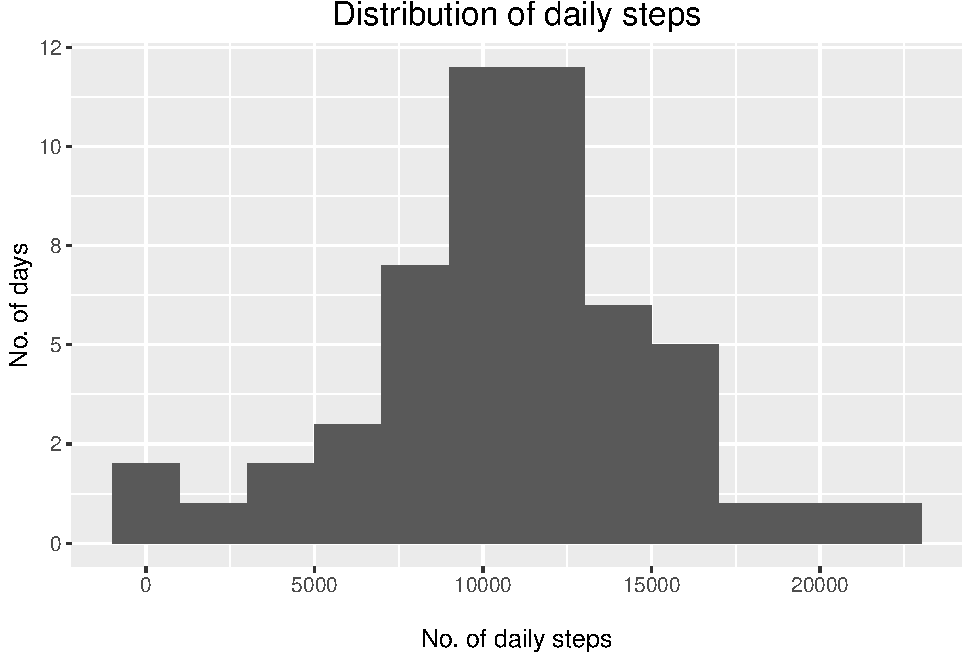
\includegraphics{PA1_template_files/figure-latex/histo-1.pdf}

\hypertarget{mean-and-median-number-of-steps-per-day}{%
\subsection{Mean and median number of steps per
day:}\label{mean-and-median-number-of-steps-per-day}}

\begin{Shaded}
\begin{Highlighting}[]
\CommentTok{\# Mean/median values}
\NormalTok{day\_mean }\OtherTok{\textless{}{-}} \FunctionTok{mean}\NormalTok{(daily}\SpecialCharTok{$}\NormalTok{total, }\AttributeTok{na.rm =} \ConstantTok{TRUE}\NormalTok{) }\SpecialCharTok{\%\textgreater{}\%} \FunctionTok{round}\NormalTok{()}
\NormalTok{day\_median }\OtherTok{\textless{}{-}} \FunctionTok{median}\NormalTok{(daily}\SpecialCharTok{$}\NormalTok{total, }\AttributeTok{na.rm =} \ConstantTok{TRUE}\NormalTok{) }\SpecialCharTok{\%\textgreater{}\%} \FunctionTok{round}\NormalTok{()}
\end{Highlighting}
\end{Shaded}

Mean steps taken per day: \textbf{10766}

Median steps taken per day: \textbf{10765}

\hypertarget{what-is-the-average-daily-activity-pattern}{%
\subsection{What is the average daily activity
pattern?}\label{what-is-the-average-daily-activity-pattern}}

\begin{Shaded}
\begin{Highlighting}[]
\NormalTok{interval\_means }\OtherTok{\textless{}{-}}\NormalTok{ odata }\SpecialCharTok{\%\textgreater{}\%}
  \FunctionTok{group\_by}\NormalTok{(interval) }\SpecialCharTok{\%\textgreater{}\%}
  \FunctionTok{summarize}\NormalTok{(}\AttributeTok{mean =} \FunctionTok{mean}\NormalTok{(steps, }\AttributeTok{na.rm =} \ConstantTok{TRUE}\NormalTok{)) }\SpecialCharTok{\%\textgreater{}\%}
  \FunctionTok{ungroup}\NormalTok{() }\SpecialCharTok{\%\textgreater{}\%}
  \FunctionTok{na.omit}\NormalTok{()}

\CommentTok{\# Take the row with highest mean (interval with highest mean steps)}
\NormalTok{interval\_max }\OtherTok{\textless{}{-}}\NormalTok{ interval\_means }\SpecialCharTok{\%\textgreater{}\%}
  \FunctionTok{slice\_max}\NormalTok{(mean, }\AttributeTok{n=}\DecValTok{1}\NormalTok{) }\SpecialCharTok{\%\textgreater{}\%}
  \CommentTok{\# Round the values.}
  \FunctionTok{round}\NormalTok{()}

\NormalTok{interval\_means }\SpecialCharTok{\%\textgreater{}\%}
  \FunctionTok{ggplot}\NormalTok{(}\FunctionTok{aes}\NormalTok{(}\AttributeTok{x =}\NormalTok{ interval, }\AttributeTok{y =}\NormalTok{ mean)) }\SpecialCharTok{+}
  \FunctionTok{geom\_line}\NormalTok{() }\SpecialCharTok{+}
  \FunctionTok{labs}\NormalTok{(}\AttributeTok{x =} \StringTok{"}\SpecialCharTok{\textbackslash{}n}\StringTok{Time interval"}\NormalTok{,}
       \AttributeTok{y =} \StringTok{"Mean steps taken per 5{-}min interval}\SpecialCharTok{\textbackslash{}n}\StringTok{"}\NormalTok{,}
       \AttributeTok{title =} \StringTok{"Mean steps taken per time interval"}\NormalTok{) }\SpecialCharTok{+} 
  \FunctionTok{my\_theme}\NormalTok{()}
\end{Highlighting}
\end{Shaded}

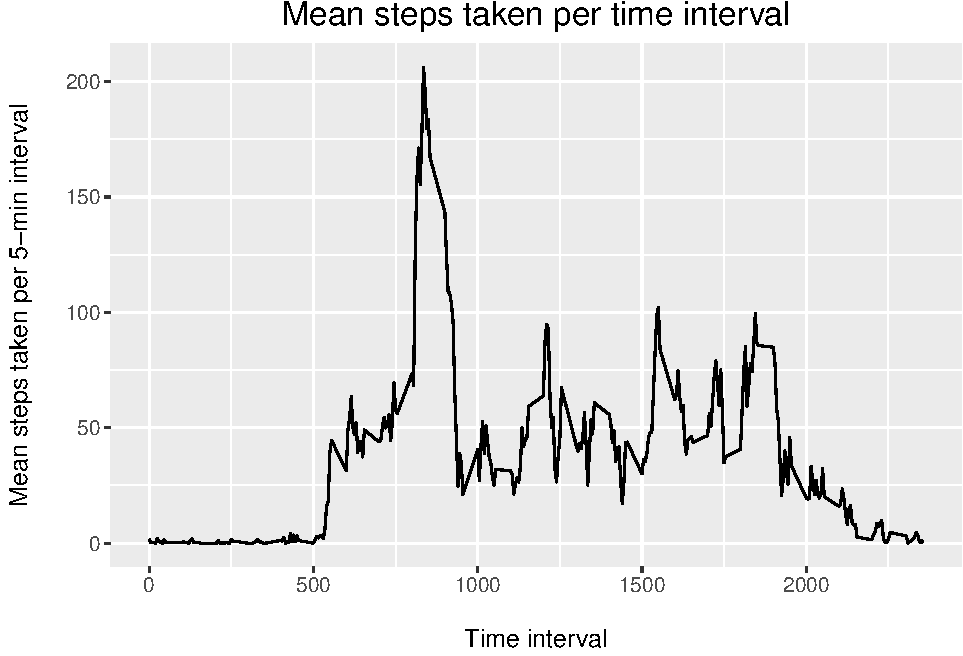
\includegraphics{PA1_template_files/figure-latex/time-series-1.pdf}

\begin{Shaded}
\begin{Highlighting}[]
\CommentTok{\# Convert interval code to time}
\NormalTok{interval\_time }\OtherTok{\textless{}{-}} \FunctionTok{id\_to\_time}\NormalTok{(interval\_max}\SpecialCharTok{$}\NormalTok{interval)}
\end{Highlighting}
\end{Shaded}

The above plot shows the number of steps taken, on average, during each
5-minute interval. During the study period, interval \#835 was the one
during which the most steps were taken--on average, 206. Interval \#835
corresponds to 08:35:00.

\hypertarget{imputing-missing-values}{%
\subsection{Imputing missing values}\label{imputing-missing-values}}

Missing data points: \textbf{2304}.

We will impute missing data with the mean value from the same intervals
in remaining days. This is under the assumption that there are
typical\textless- times of the day (e.g., 12 am through 6 am) where an
individual is likely to be at rest. We use \texttt{data.table} which
affords a good combination of execution speed and readability. Column
\texttt{imputed} in the new dataframe (\texttt{impdata}) stores
non-missing and imputed values.

\textbf{Coding environment}

Using \texttt{data.table} operations mostly as an exercise, but it
should also be the fastest option.

\begin{Shaded}
\begin{Highlighting}[]
\CommentTok{\# Loading for fast operation when imputing}
\FunctionTok{library}\NormalTok{(data.table)}

\CommentTok{\# For readability, create a "lambda" function which will go into the}
\CommentTok{\# data.table statement}
\NormalTok{impute.mean }\OtherTok{\textless{}{-}} \ControlFlowTok{function}\NormalTok{(var) }\FunctionTok{replace}\NormalTok{(var, }\FunctionTok{is.na}\NormalTok{(var), }\FunctionTok{mean}\NormalTok{(var, }\AttributeTok{na.rm =} \ConstantTok{TRUE}\NormalTok{))}
\CommentTok{\# Create data.table}
\NormalTok{impdata }\OtherTok{\textless{}{-}}\FunctionTok{setDT}\NormalTok{(odata)}

\NormalTok{impdata[,}
\NormalTok{        imputed }\SpecialCharTok{:}\ErrorTok{=} \FunctionTok{impute.mean}\NormalTok{(steps),}
\NormalTok{        by }\OtherTok{=}\NormalTok{ interval]}

\CommentTok{\# On a copy of the data, group by day and sum daily steps}
\NormalTok{histdata }\OtherTok{\textless{}{-}}\NormalTok{ impdata[,}
\NormalTok{                    .(}\AttributeTok{total =} \FunctionTok{sum}\NormalTok{(imputed)),}
\NormalTok{                    by }\OtherTok{=}\NormalTok{ date]}
\CommentTok{\# Plot histo}
\NormalTok{histdata }\SpecialCharTok{\%\textgreater{}\%}
  \FunctionTok{ggplot}\NormalTok{(}\FunctionTok{aes}\NormalTok{(}\AttributeTok{x =}\NormalTok{ total)) }\SpecialCharTok{+}
  \FunctionTok{geom\_histogram}\NormalTok{(}\AttributeTok{binwidth =} \DecValTok{2000}\NormalTok{) }\SpecialCharTok{+}
  \FunctionTok{labs}\NormalTok{(}\AttributeTok{x =} \StringTok{"}\SpecialCharTok{\textbackslash{}n}\StringTok{No. of daily steps"}\NormalTok{,}
       \AttributeTok{y =} \StringTok{"No. of days"}\NormalTok{,}
       \AttributeTok{title =} \StringTok{"Distribution of steps taken daily with imputed missing data"}
\NormalTok{       ) }\SpecialCharTok{+}
  \FunctionTok{my\_theme}\NormalTok{()}
\end{Highlighting}
\end{Shaded}

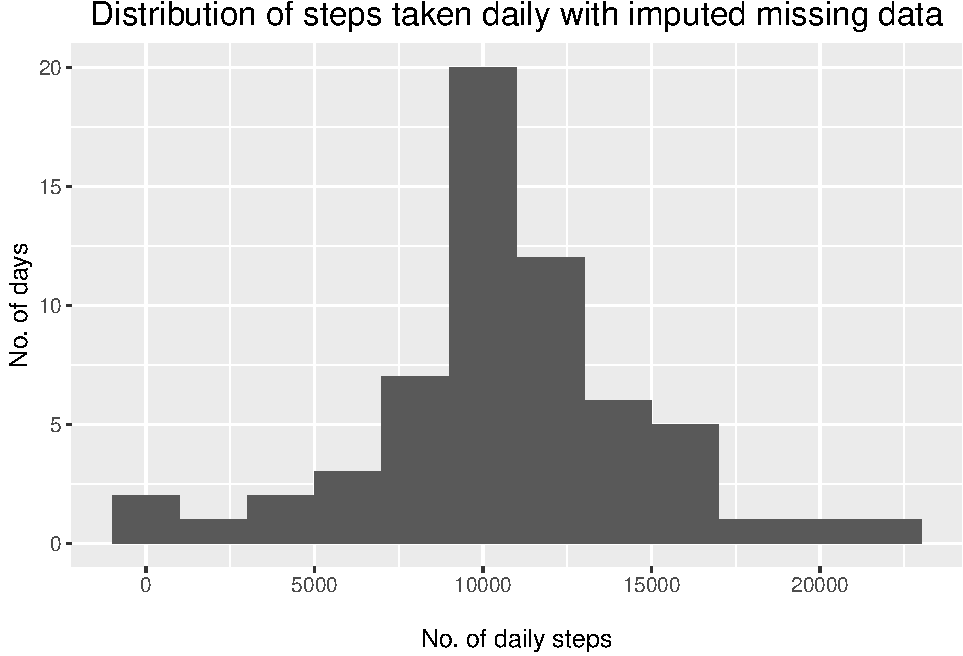
\includegraphics{PA1_template_files/figure-latex/week-analysis-1.pdf}

\hypertarget{are-there-differences-in-activity-patterns-between-weekdays-and-weekends}{%
\subsection{Are there differences in activity patterns between weekdays
and
weekends?}\label{are-there-differences-in-activity-patterns-between-weekdays-and-weekends}}

To answer this question, we will use imputed data and convert the dates
to a ``day-of-the-week'' integer (\emph{i.e.}, Monday = 1, Tuesday = 2,
\emph{etc\ldots{}}). We'll then plot the mean steps taken per 5-minute
interval during weekdays and weekends.

\begin{Shaded}
\begin{Highlighting}[]
\CommentTok{\# Get day{-}of{-}the{-}week and mark each row as "Weekdays" or "Weekends" (factor)}
\NormalTok{weekdata }\OtherTok{\textless{}{-}} \FunctionTok{setDT}\NormalTok{(}\FunctionTok{copy}\NormalTok{(impdata))}
\NormalTok{weekdata[, }\StringTok{\textasciigrave{}}\AttributeTok{:=}\StringTok{\textasciigrave{}}\NormalTok{(}\AttributeTok{day =} \FunctionTok{as.integer}\NormalTok{(}\FunctionTok{strftime}\NormalTok{(date, }\StringTok{\textquotesingle{}\%u\textquotesingle{}}\NormalTok{)))]}
\NormalTok{weekdata[, }\StringTok{\textasciigrave{}}\AttributeTok{:=}\StringTok{\textasciigrave{}}\NormalTok{(}\AttributeTok{type =} \FunctionTok{ifelse}\NormalTok{(day }\SpecialCharTok{\textgreater{}} \DecValTok{5}\NormalTok{, }\StringTok{"Weekends"}\NormalTok{, }\StringTok{"Weekdays"}\NormalTok{))]}
\NormalTok{weekdata[, type }\SpecialCharTok{:}\ErrorTok{=} \FunctionTok{as.factor}\NormalTok{(type)]}

\CommentTok{\# Time formatting function}
\NormalTok{time\_label }\OtherTok{\textless{}{-}} \ControlFlowTok{function}\NormalTok{(x) \{}\FunctionTok{strftime}\NormalTok{(x, }\StringTok{\textquotesingle{}\%H:\%M\textquotesingle{}}\NormalTok{)\}}

\CommentTok{\# Compute mean values for each 5 min{-}interval}
\NormalTok{weekdata[, }\StringTok{\textasciigrave{}}\AttributeTok{:=}\StringTok{\textasciigrave{}}\NormalTok{(}\AttributeTok{mean\_steps =} \FunctionTok{mean}\NormalTok{(imputed, }\AttributeTok{na.rm =} \ConstantTok{TRUE}\NormalTok{),}
                \AttributeTok{time =} \FunctionTok{id\_to\_time}\NormalTok{(interval)),}
\NormalTok{     by }\OtherTok{=}\NormalTok{ .(interval, type)]}
\CommentTok{\# Select columns we\textquotesingle{}re interested in}
\NormalTok{cols }\OtherTok{=} \FunctionTok{c}\NormalTok{(}\StringTok{\textquotesingle{}date\textquotesingle{}}\NormalTok{, }\StringTok{\textquotesingle{}time\textquotesingle{}}\NormalTok{, }\StringTok{\textquotesingle{}mean\_steps\textquotesingle{}}\NormalTok{)}
\CommentTok{\# Aggregate for plotting}
\NormalTok{weekdata[, .SD[1L], by }\OtherTok{=}\NormalTok{ .(interval, type), .SDcols }\OtherTok{=}\NormalTok{ cols] }\SpecialCharTok{\%\textgreater{}\%}
  
\FunctionTok{ggplot}\NormalTok{(}\FunctionTok{aes}\NormalTok{(}\AttributeTok{x =}\NormalTok{ time, }\AttributeTok{y =}\NormalTok{ mean\_steps)) }\SpecialCharTok{+}
  \FunctionTok{geom\_line}\NormalTok{() }\SpecialCharTok{+}
  \FunctionTok{facet\_wrap}\NormalTok{(}\FunctionTok{vars}\NormalTok{(type), }\AttributeTok{labeller =}\NormalTok{ label\_value) }\SpecialCharTok{+}
  \FunctionTok{labs}\NormalTok{(}\AttributeTok{x =} \StringTok{"}\SpecialCharTok{\textbackslash{}n}\StringTok{Time of day"}\NormalTok{,}
       \AttributeTok{y =} \StringTok{"Steps taken"}\NormalTok{,}
       \AttributeTok{title =} \StringTok{"Comparison of mean steps taken per interval,}\SpecialCharTok{\textbackslash{}n}\StringTok{ by weekday"}\NormalTok{,}
       \AttributeTok{subtitle =} \StringTok{"Interval IDs converted to time"}\NormalTok{) }\SpecialCharTok{+}
  \FunctionTok{scale\_x\_time}\NormalTok{(}\AttributeTok{labels =}\NormalTok{ time\_label,}
               \AttributeTok{breaks =}\NormalTok{ scales}\SpecialCharTok{::}\FunctionTok{breaks\_width}\NormalTok{(}\StringTok{\textquotesingle{}3 hours\textquotesingle{}}\NormalTok{),}
               \AttributeTok{expand =} \FunctionTok{expansion}\NormalTok{()) }\SpecialCharTok{+}
  \FunctionTok{my\_theme}\NormalTok{() }\SpecialCharTok{+}
  \FunctionTok{theme}\NormalTok{(}\AttributeTok{axis.text.x =} \FunctionTok{element\_text}\NormalTok{(}\AttributeTok{size =} \DecValTok{8}\NormalTok{))}
\end{Highlighting}
\end{Shaded}

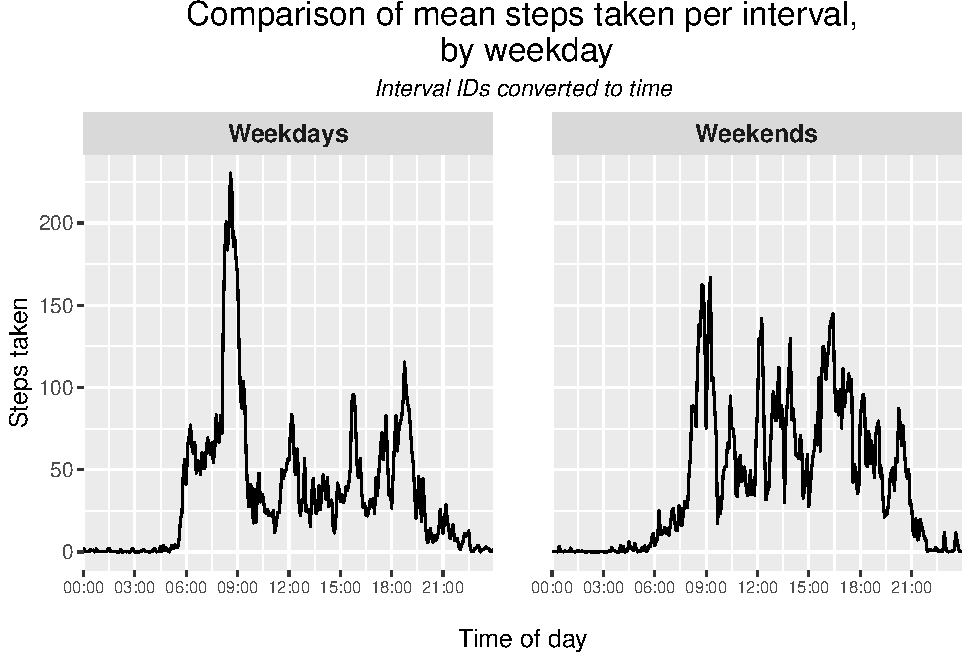
\includegraphics{PA1_template_files/figure-latex/weekday-plot-1.pdf}

\end{document}
